%%
%% This is file `sample-acmsmall.tex',
%% generated with the docstrip utility.
%%
%% The original source files were:
%%
%% samples.dtx  (with options: `all,journal,bibtex,acmsmall')
%% 
%% IMPORTANT NOTICE:
%% 
%% For the copyright see the source file.
%% 
%% Any modified versions of this file must be renamed
%% with new filenames distinct from sample-acmsmall.tex.
%% 
%% For distribution of the original source see the terms
%% for copying and modification in the file samples.dtx.
%% 
%% This generated file may be distributed as long as the
%% original source files, as listed above, are part of the
%% same distribution. (The sources need not necessarily be
%% in the same archive or directory.)
%%
%%
%% Commands for TeXCount
%TC:macro \cite [option:text,text]
%TC:macro \citep [option:text,text]
%TC:macro \citet [option:text,text]
%TC:envir table 0 1
%TC:envir table* 0 1
%TC:envir tabular [ignore] word
%TC:envir displaymath 0 word
%TC:envir math 0 word
%TC:envir comment 0 0
%%
%% The first command in your LaTeX source must be the \documentclass
%% command.
%%
%% For submission and review of your manuscript please change the
%% command to \documentclass[manuscript, screen, review]{acmart}.
%%
%% When submitting camera ready or to TAPS, please change the command
%% to \documentclass[sigconf]{acmart} or whichever template is required
%% for your publication.
%%
%%
\PassOptionsToPackage{table}{xcolor}
\documentclass[acmsmall]{acmart}
%%


\usepackage{amsmath,amsfonts}
%\usepackage{amsthm}

\usepackage{algorithmic}
\let\Bbbk\relax
\usepackage{setspace}
\usepackage{graphicx}
\usepackage{textcomp}
%\usepackage[table,xcdraw]{xcolor}
\usepackage{algorithm}
\usepackage{comment}
\usepackage{caption}
\usepackage{subcaption}
\captionsetup{compatibility=false}
\usepackage{url}
\usepackage{array}
\newcolumntype{N}{>{\centering\arraybackslash}m{.5in}}
\newcolumntype{G}{>{\centering\arraybackslash}m{1.5in}}
%\newtheorem{theorem}{Theorem}
\newcommand{\Mod}[1]{\ (\mathrm{mod}\ #1)}
%\renewcommand*{\bibfont}{\footnotesize}
%\theoremstyle{definition}
%\newtheorem{definition}{Definition}[section]
%\newtheorem{corollary}{Corollary}[theorem]


\newcommand\T{\rule{0pt}{2.6ex}}
%% \BibTeX command to typeset BibTeX logo in the docs
%\AtBeginDocument{%
%  \providecommand\BibTeX{{%
%    Bib\TeX}}}
%% Rights management information.  This information is sent to you
%% when you complete the rights form.  These commands have SAMPLE
%% values in them; it is your responsibility as an author to replace
%% the commands and values with those provided to you when you
%% complete the rights form.
\setcopyright{acmlicensed}
\copyrightyear{2018}
\acmYear{2018}
\acmDOI{XXXXXXX.XXXXXXX}

%%
%% These commands are for a JOURNAL article.
\acmJournal{JACM}
\acmVolume{37}
\acmNumber{4}
\acmArticle{111}
\acmMonth{8}

%%
%% Submission ID.
%% Use this when submitting an article to a sponsored event. You'll
%% receive a unique submission ID from the organizers
%% of the event, and this ID should be used as the parameter to this command.
%%\acmSubmissionID{123-A56-BU3}

%%
%% For managing citations, it is recommended to use bibliography
%% files in BibTeX format.
%%
%% You can then either use BibTeX with the ACM-Reference-Format style,
%% or BibLaTeX with the acmnumeric or acmauthoryear sytles, that include
%% support for advanced citation of software artefact from the
%% biblatex-software package, also separately available on CTAN.
%%
%% Look at the sample-*-biblatex.tex files for templates showcasing
%% the biblatex styles.
%%

%%
%% The majority of ACM publications use numbered citations and
%% references.  The command \citestyle{authoryear} switches to the
%% "author year" style.
%%
%% If you are preparing content for an event
%% sponsored by ACM SIGGRAPH, you must use the "author year" style of
%% citations and references.
%% Uncommenting
%% the next command will enable that style.
%%\citestyle{acmauthoryear}


%%
%% end of the preamble, start of the body of the document source.
\begin{document}

%%
%% The "title" command has an optional parameter,
%% allowing the author to define a "short title" to be used in page headers.
\title{An Efficient Approach to Store and Access Wikipedia's Revision History for Large-Scale Analysis}

%%
%% The "author" command and its associated commands are used to define
%% the authors and their affiliations.
%% Of note is the shared affiliation of the first two authors, and the
%% "authornote" and "authornotemark" commands
%% used to denote shared contribution to the research.
\author{Amit Arjun Verma}
\email{amitkumar@guvi.in}
\orcid{0000-0002-2392-0198}
\affiliation{%
  \institution{Guvi Geek Network}
  \city{IIT Madras Research Park}
  \country{India}
}

\author{Simran Setia}
\affiliation{%
  \institution{Thapar Institute of Engineering \& Technology}
  \country{India}}
\email{simran.setia@thapar.edu}

%%
%% By default, the full list of authors will be used in the page
%% headers. Often, this list is too long, and will overlap
%% other information printed in the page headers. This command allows
%% the author to define a more concise list
%% of authors' names for this purpose.
\renewcommand{\shortauthors}{Amit Arjun Verma \& Simran Setia}

%%
%% The abstract is a short summary of the work to be presented in the
%% article.
\begin{abstract}
The history-based content present on Wikipedia has served as a valuable resource for a wide range of research efforts in the field of Natural Language Processing (NLP). Due to the dynamic and ever-evolving nature of Wikipedia, conducting any large-scale temporal analysis inherently requires the ability to efficiently retrieve and process historical versions of articles. However, one of the major challenges in this domain stems from the absence of robust and scalable tools capable of handling the vast volume of revision data that Wikipedia provides. This limitation often becomes a significant bottleneck in both data management and downstream applications.

In this work, we present a comprehensive analysis of online algorithms designed specifically to address this issue by enabling efficient compression and retrieval of Wikipedia’s revision history. Our methods are supported by theoretical guarantees, demonstrating their ability to achieve high compression rates while maintaining favorable time and space complexity trade-offs. The analysis emphasizes the practicality and efficiency of our approach in scenarios where memory and processing time are constrained.

Furthermore, we conduct experiments on a set of sampled Wikipedia articles, applying our online parameter extraction method. The results reveal that our algorithm is capable of compressing the dataset to as little as 6\% of its original size—achieving up to 94\% compression. To the best of our knowledge, this work represents the first detailed and rigorous attempt to analyze and quantify the compression of Wikipedia’s complete revision history dataset, setting the stage for more scalable and efficient NLP applications based on historical web data.
\end{abstract}

%%
%% The code below is generated by the tool at http://dl.acm.org/ccs.cfm.
%% Please copy and paste the code instead of the example below.
%%
\begin{CCSXML}
<ccs2012>
   <concept>
       <concept_id>10002951.10003317.10003371</concept_id>
       <concept_desc>Information systems~Specialized information retrieval</concept_desc>
       <concept_significance>500</concept_significance>
       </concept>
   <concept>
       <concept_id>10002951.10003317.10003347.10003352</concept_id>
       <concept_desc>Information systems~Information extraction</concept_desc>
       <concept_significance>300</concept_significance>
       </concept>
   <concept>
       <concept_id>10002951.10003260.10003277.10003279</concept_id>
       <concept_desc>Information systems~Data extraction and integration</concept_desc>
       <concept_significance>300</concept_significance>
       </concept>
   <concept>
       <concept_id>10002951.10003227.10003392</concept_id>
       <concept_desc>Information systems~Digital libraries and archives</concept_desc>
       <concept_significance>300</concept_significance>
       </concept>
 </ccs2012>
\end{CCSXML}

\ccsdesc[500]{Information systems~Specialized information retrieval}
\ccsdesc[300]{Information systems~Information extraction}
\ccsdesc[300]{Information systems~Data extraction and integration}
\ccsdesc[300]{Information systems~Digital libraries and archives}


%%
%% Keywords. The author(s) should pick words that accurately describe
%% the work being presented. Separate the keywords with commas.
\keywords{Wikipedia, Edit-History, Information-retrieval, Datasets, Natural Language Processing, Compression, Algorithm}

\received{20 February 2007}
\received[revised]{12 March 2009}
\received[accepted]{5 June 2009}

%%
%% This command processes the author and affiliation and title
%% information and builds the first part of the formatted document.
\maketitle

\section{Introduction}\label{Intro}
Over the past decade, Wikipedia, the free online collaborative encyclopedia, has been a subject of enormous interest in the various research domains~\cite{zhu2014impact,gabrilovich2006overcoming,mestyan2013early}. The intense collaboration on Wikipedia and its open dataset have attracted researchers to study various tasks such as to study online collaboration dynamics~\cite{kittur2008harnessing, gallus2020gender, zhang2017crowd, israeli2024test, jurgens2012temporal}, to examine its impact on other online collaborative portals~\cite{vincent2018examining, marashi2013impact, piccardi2021value}, and to predict the box office collection~\cite{mestyan2013early}. Furthermore, the rich content of Wikipedia has been used for numerous NLP tasks, e.g., training Large Language Models~\cite{roberts2020much, jang2022temporalwiki,su2024wikiformer}, generating word embeddings~\cite{mikolov2013efficient,bojanowski2017enriching, giesen2022leveraging, berenguer2024word}, semantic relatedness measures~\cite{gabrilovich2007computing}, or text categorization~\cite{gabrilovich2006overcoming}.

At the core of all the mentioned research lies the Wikipedia dataset. Wikipedia is not a static repository of knowledge—it is a dynamic, ever-evolving platform where millions of users collaboratively contribute by making edits across articles. Each and every edit made to an article is preserved in its edit history, capturing the trajectory of knowledge construction over time. This history is comprehensively archived and made publicly available in the form of full XML dumps, where each article includes multiple distinct versions known as \emph{revisions}. On average, there are 18.93 revisions per article, as reported by \cite{wikirev}. Each revision is stored incrementally—meaning it is composed of the preceding revision along with the newly introduced changes. While this format allows the precise reconstruction of the article’s development, it also leads to a significant accumulation of redundant information across revisions. As a result, the storage size of individual articles can quickly grow to several megabytes or even gigabytes, depending on the frequency and size of the edits. This exponential increase in data volume makes it computationally expensive and time-consuming to conduct large-scale analyses involving the complete revision history. Since most Wikipedia-based research depends on tracking and comparing revisions to study patterns, behaviors, or content evolution, this massive data size becomes a major bottleneck in efficiently carrying out such tasks.

Even with well maintained open Wikipedia dataset and advanced computational power, Wikipedia edits extraction is costly in time and space complexity. Also, extracting and processing Wikipedia's full revision history is difficult and time-consuming for the end-users. For instance, according to Milne et al.~\cite{milne2013open}, a significant amount of effort is required to mine and preprocess the dataset of Wikipedia.
This paper presents a novel method to represent the Wikipedia full revision history by optimally storing the edit history. Based on this optimal representation, we present an algorithm to efficiently extract the edits by reconstructing a specific past state of Wikipedia from its edit history. 

The rationale behind data compression is to store the edits made in the current revision exclusively. This compression is relatively simple and can be achieved by taking the \emph{difference} of the current revision with the previous one using the diff algorithm \cite{hunt1976algorithm}.  If all the revisions are compressed by storing only the difference, the revision access time will increase as each revision will require reconstructing the text from a list of changes. It is evident that there is a trade-off between the retrieval time and the compression of revisions. Thus, to accelerate the reconstruction process, every $k^\text{th}$ revision is stored as a full revision. A similar approach was followed by Ferschke et al. \cite{ferschke2011wikipedia}, where the value of $k$ (interval length) was fixed to 1000 irrespective of input article. Following the lines of Ferschke et al.'s work, Verma et al.~\cite{verma2021open} proposed a method for compressing the revision history using the interval length $k=\sqrt{n}$. 

We propose an online algorithm to compress and retrieve the Wikipedia article's revisions, which can scale up with the Wikipedia dataset size. We show that our approach outperforms the previously established methods in terms of retrieval time and space complexity. Moreover, the dataset consisting of the compressed representation of Wikipedia articles' full revision history will be a novel source of knowledge for Wikipedia-based analysis. The articles' full revision history can be used to train a model for vandalism detection~\cite{chin2010detecting}, to identify semantic edit intentions~\cite{yang2017identifying}, to extract semantic information from Wikipedia~\cite{tran2017hedera}, to identify editor's role in Wikipedia~\cite{yang2016did}, to correct grammatical errors~\cite{boyd2018using}, or to create longitudinal Wikipedia link network~\cite{consonni2019wikilinkgraphs}. With the proposed algorithm, we reduce the required storage space to less than 7\% of its original size. We validate our results empirically on a sampled Wikipedia full revision history dataset. We also compare the space and time complexity of our method with Ferschke et al.'s method.	

The rest of the paper is structured to guide the reader through the background, methodology, and results of our work in a logical and coherent manner. We begin by presenting a review of the relevant literature, which includes an overview of existing research efforts and a discussion of various tools and APIs available for retrieving and interacting with Wikipedia's dataset (Section 2). This section sets the foundation for understanding the current landscape of Wikipedia-based data access and analysis. Next, we formally introduce the structure of Wikipedia's edit history and lay out the key preliminaries necessary to comprehend the underlying concepts used in our approach (Section 3). This includes a detailed explanation of the revision format and the challenges involved in processing the full edit history.

Building upon this formal groundwork, we proceed to describe our proposed algorithm in detail, including the step-by-step methodology and the theoretical analysis that supports its design and effectiveness (Section 4). This section provides both the intuition and mathematical justification behind our approach. Finally, we transition into the experimental evaluation of our method. We present comprehensive results that demonstrate the performance and efficiency of our approach, including comparisons with existing techniques. This evaluation is covered in Sections 5 and 6, where we analyze both the practical applicability and the empirical benefits of our method through rigorous experimentation.
  

\section{Related Work}\label{RelWork}
Accessing Wikipedia data has always been challenging. A significant amount of effort is required to mine and preprocess the Wikipedia dataset \cite{milne2013open}. Many APIs and toolkits have been developed to solve the Wikipedia data extraction issue. These APIs and toolkits are categorised into two sub-classes. The first class consists of libraries and toolkits, which depend on Wikipedia live database for all the queries. On the other hand, the second class comprises toolkits that parse the Wikipedia XML dump to retrieve the edit history. In this section, we describe a few of these APIs and methods closely related to our work. 

\subsection{Wikipedia-based parsers}
One possibility to retrieve the Wikipedia revision history is to parse the Wikipedia XML dump manually. However, due to these dump's massive size, efficient access to the edit history is infeasible. To solve this issue, various tools to extract and parse the Wikipedia data dump are available. For instance, Verma et al.~\cite{vermakdap} developed a python based library named KDAP (Knowledge Data Analysis and Processing Platform) to extract and analyze the dataset of online collaborative portals, including Wikipedia. The library efficiently retrieves the edit history by parallelly parsing through the multiple Wikipedia articles' revision history and optimizing time and space complexity. However, it requires one to download each article's full revision history and store it in the local machine. Even with the parallel processing, parsing a broad set of articles is infeasible. Wikibrain~\cite{sen2014wikibrain} is another example of data dump parser which provides state-of-the-art algorithms ranging from extracting pageviews to finding semantic relatedness, but the number of extraction algorithms is limited. Various other parsers provide similar parsing features (e.g., MediaWiki Utilities~\cite{Halfaker1}, mwxml~\cite{Halfaker2}), but requires full revision history dataset. Similar to general analysis toolkits, application specific tollkits are also available to extract and parse the Wikipedia data. For instance, WikiMirs~\cite{hu2013wikimirs} is a retrieval toolkit to extract the mathematical formulas from the Wikipedia articles. 

As mentioned above, of all the existing toolkits, we wish to highlight Wikipedia Revision Toolkit developed by Ferschke et al. \cite{ferschke2011wikipedia}. The toolkit represents Wikipedia revisions in a compressed form by storing the edits, achieving a compression up to 98\%. Efficient retrieval methods were implemented to retrieve the data of a particular revision from the compressed data dump. However, the compression and retrieval methods do not scale up with the current size of the dataset. Moreover, the authors did not discuss the theoretical analysis of choosing a fixed length of 1000. Given that Wikipedia's size is increasing with time, fixing the interval length as 1000 may result in inefficient compression. Verma et al.~\cite{verma2021open} in their toolkit extended Ferschke's compression method by emperically showing that the interval-length of $\sqrt{n}$ gives the ideal compression ratio. However, no theoretical analysis was provided.


\begin{figure}
    \centering
    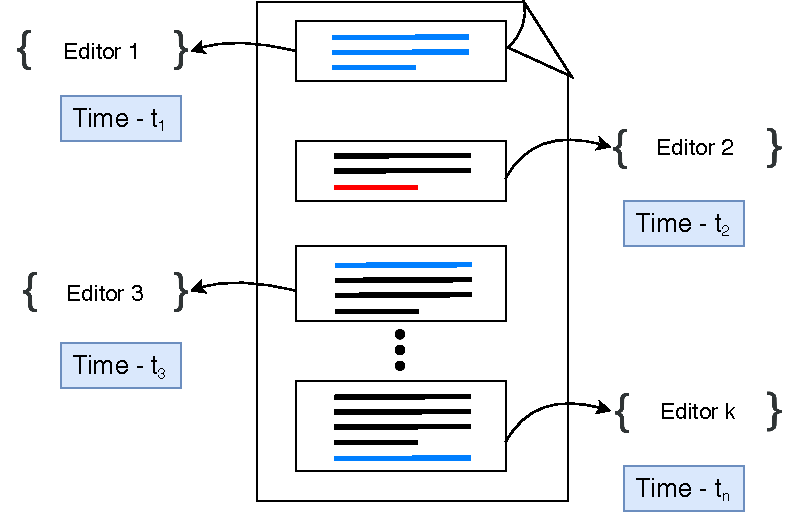
\includegraphics[scale=0.7]{sequential_knowledge.pdf}
    \caption{An illustration of sequential knowledge building in collaborative environment. A contribution can be seen in the form of addition (blue) or deletion (red) information. The blue lines represent the content that were added in that revision, whereas the red lines represent the content which were deleted in that revision. The black lines shows the content which stayed from the previous revision. Best viewed in color.}
    \label{fig:seq}
\end{figure}

\subsection{Wikipedia-based APIs}
Apart from manually parsing the dataset--which is inefficient given the vast size of the data dump--one can use the existing \emph{APIs} (such as MediaWiki\footnote{\url{https://www.mediawiki.org/wiki/API}} and Wikipedia Query Service\footnote{\url{https://query.wikidata.org/}}) which directly queries the Wikipedia database. A typical example of such a tool is the web-based Wikipedia API. It has been frequently used to find articles related to a word~\cite{wu2015sense}, retrieve language links~\cite{steiner2013mj}, or extract details about edits in articles~\cite{boukhelifa2010real}. However, being a web-based API, a particular revision must be requested from the service, transferred over the Internet, and stored locally in an appropriate format. A similar tool is the Wikipedia Query Service, which helps user query against the wikidata\footnote{https://www.wikidata.org/wiki/Wikidata:Main\_Page} dataset.

For a large scale analysis, APIs that store the Wikipedia data into a local database system are best suited. However, current database-based APIs do not support the retrieval of edit history. For example, \emph{Wikipedia Miner}~\cite{milne2013open} provides a preprocessed database by representing the articles, categories, and redirects as Java classes. Although the API provides the retrieval of Wikipedia in a structured format, it makes little use of the articles' textual content. Another API for retrieving the Wikipedia dataset using a preprocessed database is \emph{JWPL}~\cite{zesch2008extracting}. Besides retrieving the structured data from Wikipedia, it also has a MediaWiki markup parser to extract the data from unstructured text further.



\section{Background}
Prior to presenting our proposed method, we first provide a higher-level description of the Wikipedia edit-history dataset. We also formally define the Wikipedia edit mechanism as a preliminary for our work.
\subsection{Wikipedia Edit History}
Being a crowd-sourced portal, Wikipedia maintains each of its article's development in terms of \emph{revision history} (edit history)\footnote{These two terms are synony-mous and essentially interchangeable}. Chhabra et al.~\cite{chhabra2017does} describes the knowledge building process in Wikipedia as a \emph{sequential} process, where a single user's contribution is added at a particular time-stamp. Wikipedia records all the edits of an article along with other details such as user id, time-stamp, and bytes. Fig. \ref{fig:seq} describes the knowledge development on a Wikipedia article. As illustrated in the figure, each revision of a Wikipedia article is a combination of previous revision and the current edits. Wikipedia regularly dumps the full revision history of all the articles in XML format. Each article's XML dump contains all the edits in the form of revisions and information such as editor's id, time-stamp, revision size, and comments. We will now formally define the revision mechanism of Wikipedia.
         

\subsection{Preliminaries}\label{pre}
Being a crowd-sourced portal, Wikipedia maintains each of its article's development in terms of \emph{revision history} (edit history)\footnote{These two terms are synonymous and essentially interchangeable}. Chhabra et al.~\cite{chhabra2017does} describe the knowledge-building process in Wikipedia as a \emph{sequential} process, where a single user's contribution is added at a particular time-stamp. Wikipedia records all the edits of an article along with other details such as user ID, time-stamp, and bytes. Each revision of a Wikipedia article is a combination of previous revisions and the current edits.
Assume there are $n$ revisions for a Wikipedia article, define $\mathcal{R} =\{r_i \mid r_i \text{ is the } i^{\text{th}} \text{revision}, 0 \leq i \leq n\}$ to be the set of all $n$ revisions of the article, where $r_0$ denotes the empty revision. $\mathcal{R}$ can also be considered as the XML dump of a Wikipedia article.
%\textcolor{blue}{(XML dump can be mentioned in the background. Done!)}. 
Let $dr_{i}$ denote the difference between two consecutive revisions $i$ and $i-1$ i.e., $dr_i = r_{i} \ominus r_{i-1}$, where $\ominus : \mathcal{R}\times\mathcal{R}\rightarrow d\mathcal{R}$ is the \emph{diff} operator which is defined as the smallest set of deletions and insertions required to create one text from the other~\cite{hunt1976algorithm}. Thus, $d\mathcal{R}$ is the set of all \emph{difference} revision obtained from \emph{diff} operator. Since edits made in the current revision results in the successive revision, $r_{i}$ can also be written as $r_{i} = r_{i-1} \oplus dr_{i}$, where $\oplus : \mathcal{R} \times d\mathcal{R} \rightarrow \mathcal{R}$ restores one of the revisions that generated $dr$, acting as a \emph{decompressor}.
%Here are two different methods of compressing and decompressing the Wikipedia data:


%\subsection{Method 1}\label{method 1}
One way of storing the data is to store only the difference $dr_i$, $\forall i \in \left[1, n\right]$ rather than the entire revision. Though this results in significant amount of compression, the reconstruction time of a particular revision is more than its uncompressed counterpart. A revision $r_i$ can be retrieved by loading $d\mathcal{R}$ to the main memory and recursively constructing $r_1$, $r_2$, $\cdots$, $r_i$ using $dr_1$, $dr_2$, $\cdots$, $dr_{i-1}$ respectively, i.e.,
\begin{equation*}
\underbrace{dr_1} \oplus dr_2 \oplus dr_3 \oplus \cdots dr_i
\end{equation*}
\begin{equation*}
  =\underbrace{r_1 \oplus dr_2} \oplus dr_3 \oplus \cdots dr_i
\end{equation*}
\begin{equation*}
=\underbrace{r_2 \oplus dr_3} \oplus \cdots dr_i
\end{equation*}
\begin{equation*}
    \ddots
\end{equation*}
\begin{equation*}
    = r_i
\end{equation*}

Moreover, the reconstruction time and compression ratio depend on the type of algorithm used to compute the \emph{diff} between the two revisions. Much research has been conducted on developing efficient difference algorithms. However, both their runtime and the size of the resulting output are not feasible given the massive redundancy in Wikipedia's articles' revisions. For instance, Heckel's~\cite{heckel1978technique} algorithm for computing difference is quick but provides inefficient output if related text exists in the inputs. Similarly, the algorithm provided by MacDonald~\cite{macdonald2000file} uses copy and insert operators to compute the difference. The copy operator is used to copy the text to the output whenever an exact match is found, which again is infeasible given the size and redundant text in Wikipedia. Arguably the best difference algorithm for our purpose is proposed by Mayer~\cite{myers1986ano}, which provides the difference between two texts as a set of inserts and deletes. The algorithm takes a greedy approach by maximizing the consumption of similar lines before making any change and preferring deletions over insertions when given a choice. This approach allows the algorithm to detect redundant information while optimizing time complexity efficiently. Given two strings A and B, the algorithm takes $\mathcal{O} (nd)$ in time and space, where $n$ is the sum of the lengths of A and B and $d$ is the size of the minimum edit script for A and B. We use Mayer's algorithm to compute the difference between two revisions.
    

At any time, \textit{only} $r_{k-1}$ is stored in the main memory while reconstructing $r_k$ $(2 \leq k \leq n)$. In the worst case (retrieving the last revision), this method require $\mathcal{O}(nd+(m+d))$ in space, and $\mathcal{O}(n(m+d))$ in time, where $m$ is the maximum size of the revision in $\mathcal{R}$ and $d$ is the maximum size of the \emph{difference} revision in $d\mathcal{R}$. This is because, the reconstruction of the text $r_{i+1}$ from $r_i$ and $dr_i$ would require $\mathcal{O}(||r_i||+||dr_i||)$ in space and time, 
%and $\mathcal{O}(||r_{i+1}||)$
where $||\cdot||$ denote the size of the text (please refer to text reconstruction from diff patch~\cite{diffpatch}).

%\footnote{The \emph{diff} algorithm performs quadratic in time in the worst case and has expected-case behavior dependent in a complicated way on how many elements the sequences have in common; best case time is linear.}

\begin{table*}[]
\centering
\caption{Representation of difference between every two consecutive revisions. $mr_i$ and $tr_i$ represents the memory cost saved by storing the difference $dr_i$ and the time cost to retrieve the revision $r_i$ using $r_{i-1}$ and $dr_i$, respectively. $l_i = ||r_i||$ represents the revision length of $i^{th}$ revision and $|.|$ represents the modulus function.}
\label{tab:diff_cost}
\scalebox{0.8}{
\begin{tabular}{c|ccccccc}
revisions    & $l_1$ & $l_2$                   & $l_3$                   & $l_4$                   & ... & $l_{n-1}$                         & $r_n$                     \\ \hline
differences  &    & $dl_1 = |l_2 - l_1|$            & $dl_2 = |l_3 - l_2|$            & $dl_3 = |l_4 - l_3|$            & ... & $dl_{n-1} = |l_{n-1} - l_{n-2}|$                & $dl_{n-1} = |l_{n} - l_{n-1}|$            \\
memory cost saved &    & $mr_1 = l_2-dl_1$ & $mr_2 = l_3-dl_2$ & $mr_3 = l_4-dl_3$ & ... & $mr_{n-1} = l_{n-1}-dl_{n-1}$ & $mr_{n-1} = l_n-dl_{n-1}$ \\
time cost    &    & $tr_1 = l_1+dl_1$         & $tr_2 = l_2+dl_2$         & $tr_3 = l_3+dl_3$         & ... & $tr_{n-2} = l_{n-2}+dl_{n-2}$           & $tr_{n-1} = l_{n-1}+dl_{n-1}$  \\ \hline      
\end{tabular}}
\end{table*}

\section{Wikipedia Data Compression and Decompression: An Efficient Way}\label{WikiComp}
This section provides an analysis of our approach for efficiently compressing and retrieving Wikipedia's edit history. Based on our method, we provide algorithms to perform both random and full edit history extraction.  
\subsection{Fixed-Interval Length Compression}
We develop a generalized model that calculates the interval length ($k$) based on the input file, optimizing both the time and space complexity. Here, we modify the set $d\mathcal{R}$ into $\Tilde{d\mathcal{R}}$, the set of difference between two consecutive revisions except at multiples of estimated $k \in [1, n]$. Each element of $\Tilde{d\mathcal{R}}$, $\Tilde{dr_i}$, is defined as:
\begin{equation*}
    \Tilde{dr_i} = 
    \begin{cases}
    r_{i} \ominus r_{i-1} &\quad \text{if $i \Mod{k} \neq 0$}\\
    r_{i} &\quad \text{if $i \Mod{k} = 0$}
    \end{cases}
\end{equation*}

Out of $n$ revisions, there are $\left\lfloor \dfrac{n}{k} \right\rfloor$ number of revisions that are stored as full revisions and $n-\left\lfloor \dfrac{n}{k} \right\rfloor$ number as \emph{difference} revisions. The decompression technique is same as described in the previous section except that $\Tilde{d\mathcal{R}}$ is stored in the main memory instead of $d\mathcal{R}$, which makes it $\mathcal{O}\left(\dfrac{n}{k}m + \left(n-\dfrac{n}{k}\right)d + (m+d)\right)$ in space and $\mathcal{O}(k(m+d))$ in time in the worst case (for retrieving any $i^{th}$ revision). We are able to achieve this by hashing the revisions stored as full revision, where \emph{keys} are revision number and \emph{values} are the text associated with it.

As we increase the size of the interval length, $k$, the memory space decreases and the retrieval time increases. Hence, there is a trade-off in using extreme $k$ values, giving us a chance to find the optimal $k$ (in terms of both space and time combined). Using the above two expressions, given an XML dump of a Wikipedia article, we can compress the data with a value of $k$.

%$k = \mathcal{O}(\sqrt{n}$).


\begin{comment}
\begin{table*}[th]
\centering
\caption{Comparison of compression methods using various interval lengths based on revision retrieval time and compression ratio.}
\label{tab:compress}
\begin{tabular}{cccccccc}
\hline \T
                                         & \multicolumn{4}{c}{\textbf{Time (seconds)}}                                                                     & \multicolumn{1}{l}{} & \multicolumn{2}{c}{\textbf{Memory}}                       \\ \cline{2-5} \cline{7-8} \T
\textbf{Interval Length}                 & \multicolumn{2}{c}{\textbf{Full Revision Extraction}} & \multicolumn{2}{c}{\textbf{Random Revision Extraction}} & \multicolumn{1}{l}{} & \multicolumn{2}{c}{\textbf{Original to Compressed Ratio}} \\ \hline \T
                                         & \qquad \textbf{avg}              & \quad \textbf{std}              & \qquad \textbf{avg}               & \quad \textbf{std}               &                      & \qquad \textbf{avg}                & \quad \textbf{std}                \\ \hline \\
\textbf{$k = 2$}                           & \qquad 0.087                     &\quad 0.587                     &\qquad 0.008                      &\quad 0.011                      &                      &\qquad 0.566                       &\quad 0.075                       \\ \T
\textbf{$k = \sqrt{\frac{n(m-d)}{m+d}}$} & \qquad 0.087                     &\quad 0.586                     &\qquad 0.080                      &\quad 0.239                      &                      &\qquad 0.174                       &\quad 0.126                       \\ \T
\textbf{$k = \sqrt{n}$}                  & \qquad 0.087                     &\quad 0.589                     &\qquad 0.090                      &\quad 0.271                      &                      &\qquad 0.166                       &\quad 0.113                       \\ \T
\textbf{$k = 1000$}                      & \qquad 0.089                     &\quad 0.601                     &\qquad 1.290                      &\quad 1.65                       &                      &\qquad 0.114                       &\quad 0.096                       \\ \T
\textbf{$k = n-1$}                       & \qquad 0.089                     &\quad 0.614                     &\qquad 2.254                      &\quad 5.163                      &                      &\qquad 0.103                       &\quad 0.091                       \\ \hline
\end{tabular}
\end{table*}
\end{comment}

\begin{theorem}
For a given Wikipedia article with $n$ (total number of revisions), $m$ (maximum size of the revision in $\mathcal{R}$) and $d$ (maximum size of the \emph{difference} revision in $d\mathcal{R}$), the optimal $k$ is $\sqrt{n\left(\dfrac{m-d}{m+d}\right)}$.
\end{theorem}

\begin{proof}
Since for any given article we have $n$, $m$ and $d$ as constants, the minima of the function $f(k) = \dfrac{nm}{k} + nd - \dfrac{nd}{k} + (m+d) + k(m+d)$ needs to be calculated. Differentiating the function $f(k)$ with respect to $k$ and equating it to zero, we get the desired $k$. It can be easily verified that the obtained $k$ is the minima of $f(k)$.\\

\end{proof}

If we let $k = 1$, then the compression method discussed above is the same as the XML dump of an article. On the other hand, if $k = n$, the method reduces to storing only the \emph{difference} revisions, as discussed in preliminaries, making this a general method. Based on our analysis, we now provide an efficient revision extraction algorithm for compressed Wikipedia dataset. 

\subsection{Variable-Interval Length Compression}
The above method stores the difference between two consecutive revisions except for a few fixed intervals ($k$). Although the above method reduces the overall compression ratio and the random revision retrieval time, the fixed interval length restricts us from optimal compression. We modify the above method by storing the full revisions at variable interval lengths. Our goal using the variable-length intervals is to store the difference only when there is a minor edit, in turn optimizing the overall compression. We translate this optimization problem into an ordered set partition problem. More specifically, for a Wikipedia article, we define $S = \{s_i \mid s_i = ||r_i||, 0 \leq i \leq n \}$ as an ordered set of revision sizes, where $||r_i||$ represents the text length of revision $r_i \in \mathcal{R}$. For simplicity's sake assume $||r_{i} \ominus r_{i-1}|| = |s_i - s_{i-1}|$ ($|.|$ is the absolute function), which means we can compute $||dr_{i}|| = |s_i - s_{i-1}|$ (we will relax this assumption later). Given a set $S$ for a corresponding Wikipedia article, we define $P$ as a partition of the set $S$ such that:


\begin{itemize}
	\item $P = \{p_1, p_2, p_3, \ldots, p_N\}$, where $N \leq n$.
	\item $p_j$ (for some $j$) is either a singleton set or if $s_l, s_m \in p_j $ and if $l < m$, then $s_i \in p_j\ \forall i \in (l,m)$.
	\item Given $p_j = \{s_i \mid l\leq i\leq m\}$, we define function $f^-$ on $p_j$ as
  
$$f^-(p_j) =
\begin{cases}
s_i,  & \text{if $p_j$ is a singleton} \\
s_l + \sum_{i=l}^{m-1} |s_{i+1} - s_i|, & \text{otherwise}
\end{cases}$$

	\item Given $p_j = \{s_i \mid l\leq i\leq m\}$, we define function $t$ on $p_j$ as
  
$$t(p_j) =
\begin{cases}
1,  & \text{if $p_j$ is a singleton} \\
1 + \sum\limits_{i=l}^{m-1} s_i + |s_{i+1} - s_i|, & \text{otherwise}
\end{cases}$$
\end{itemize}

Given the partition and the function definition, the summation $\sum f^-(p_j), \forall j \in N$ represents the overall size of the set $S$ (i.e. size of the Wikipedia article) after compression. Consider a simple example where a Wikipedia article contains only three revisions and their sizes are $r_1 = 1$, $r_2 = 2$, and $r_3 = 8$. Given the size of each revision, we can represent the set $S = \{1, 2, 8\}$. If we partition this set $S$ such that $P = \{\{1\}, \{2, 8\}\}$ then $\sum f^-(p_j)$ will be 9, which we refer as the total \emph{space cost}. But what about the revision retrieval time? As explained in section \ref{pre}, given a revision $r_i$ and the difference $d_i = r_{i} \ominus r_{i+1}$, retrieving the revision $r_{i+1}$ will take $\mathcal{O}(||r_i||+||dr_i||)$ time. Which means that overall \emph{time cost} for a given set $S$ will be $\sum t(p_j), \forall j \in N$ (in the case of $S = \{1, 2, 8\}$, the time cost is 11, $\mathcal{O} (1)$ unit for $r_1$ and $r_2$, whereas $\mathcal{O} (2 + 6)$ for $r_3$). Can we define a partition in this set $S$ which minimizes the overall time cost and the space cost?

Now provided a set $S$, the problem reduces to finding a partition $P$ such that the overall time cost and the space cost are minimized. More specifically:

\begin{itemize}
	\item $\sum f^-(p_j), \forall j \in N$ is minimized and,
	\item $\sum t(p_j), \forall j \in N$ is minimized.
\end{itemize}


However, the optimization function as the summation of space and time cost ($\sum f^-(p_j) + \sum t(p_j), \forall p_j \in P$) provides a solution other than the original arrangement of the set S, only if there exist at least two consecutive revisions having the difference precisely equal to 1 (please refer to the appendix of a detailed example\footnote{\url{shorturl.at/emwEZ}}). Moreover, the solution is never unique. To overcome this challenge, we convert the optimization problem into a memory cost minimization problem based on a fixed time cost. More specifically, given a set $S$ and a fixed time cost (as a function of $n = |S|$), the optimization problem reduces to finding a partition $P$ that minimizes the overall space cost.

We first start with computing the differences between all the consecutive revisions. As illustrated in Table \ref{tab:diff_cost}, we compute the \emph{memory cost saved}  as $mr_i = ||dr_i|| - ||r_{i-1}||$, whereas the \emph{time cost} represents the time units required to retrieve a specific revision. Given a fixed time cost, we aim to maximize the memory cost saved. It is easy to verify that this maximization problem can be translated into the 0/1 knapsack problem, where the \emph{time cost} is the knapsack size, and the \emph{memory cost saved} is the profit. We now formally define the 0/1 knapsack problem and show the reduction of our partitioning problem to the 0/1 knapsack problem.


\subsubsection{0/1 knapsack definition}
Given a set $I$ of $n$ items, with each item $i \in [n]$ having a cost $c_i \in \mathbb{Z^+}$ and a value $v_i \in \mathbb{Z^+}$ associated with it, find a subset $I_{opt} \subseteq I$ of items whose cost $cost(I_{opt}) = \sum_{i \in I_{opt}} c_i$ is smaller than a defined capacity $W$ and whose value $value(I_{opt}) \in \sum_{i \in I_{opt}} v_i$ is maximal.   

Apprantly the solution to the 0/1 knapsack problem is computed through a dynamic programming approach. More specifically, we define $c[i,w]$ to be the maximum value that can be attained with capacity less than or equal to $w$ using items up to $i$. We can define $c[i,w]$ recursively as:

\begin{equation*}
c[i,w] = \begin{cases}
		 0, &\quad\text{if } i=0 | w=0,\\
		 c[i-1, w], &\quad\text{if } w_i>w,\\ 
       {\scriptstyle max(v_i+c[i-1, w-w_i],c[i-1,w])}, &\quad\text{if } i>0 \text{ \& } w\geq w_i\\
       	\end{cases}
\end{equation*}

Similar to the 0/1 knapsack problem, we define our original set $S$ of revision sizes as the set of items. The \emph{time cost} list represents the cost associated with each item, and \emph{memory cost saved} list represents each item's value. Provided a fixed maximum time cost $C$, the optimal solution maximizing the memory cost saved (minimizing the overall memory cost) can be computed using the above recursive function. The optimum set of items $I_{opt}$ can be obtained from the final solution $c[n,W]$.  

\begin{corollary}
Given a set $S$ of revision sizes and the optimal set of items $I_{opt}$, the optimal partitioning $P = \{p_1, p_2, ..., p_k\}$ is performed such that $\forall i \in [l+1, m] \ni l<m,\ p_j = \{s_i| s_i \in I_{opt}\}$. Moreover, $\forall i \in [1, n],\ s_i \in p_j$ and $s_{i+1} \in p_{j+1}$ for some $j$, iff $s_i \in I_{opt}$ and $s_{i+1} \notin I_{opt}$.
\end{corollary}

The partitioning is performed based on the optimal set of items $I_{opt}$ computed based on the 0/1 knapsack solution. The recurrence relation of 0/1 knapsack problem guarantees to return the optimal set of items provided a fixed maximum cost. Therefore, deriving from the proof of knapsack optimization, the partitioning $P$ performed using the set $I_{opt}$ is the optimal partitioning, minimizing the overall memory cost based on the given maximum time cost. 

Returning to our original problem, we now relax the assumption of $||dr_{i}|| = |s_i - s_{i-1}|$. Instead of calculating the actual diff between two revisions as $dr_i = r_{i} \ominus r_{i-1}$, we approximate the difference size as $||dr_{i}|| = 2 . |s_i - s_{i-1}|$\footnote{We emperically found that twice of the difference yields a good approximation.}. The stated approximation allows us to calculate all the consecutive differences in linear time. It is easy to varify that even after relaxing the original assumption the algorithm returns the optimal partitioning. We experimently found that using the \emph{time cost} as $n^2$ the algorithm performes optimal compression.



\begin{algorithm}
\centering
\caption{Extract $r_i$, where  $i \in [l, l+j]$}\label{alg:comp}
\begin{algorithmic}
%  \algsetup{linenosize=\small}
%  \scriptsize
\REQUIRE $\mathcal{X}$,  $k \neq 0$ or $U = [k_1, k_2, ..., k_N]$, $l$, and $j$
\STATE $prev \leftarrow None$
\STATE $curev \leftarrow None$
\IF{$X[variable] = True$} 
\STATE $\gamma \leftarrow k_q \ni \sum \limits_{m=1}^{m=q} k_m \leq l < \sum \limits_{m=1}^{m=q+1} k_m$ \COMMENT{Calculating the nearest full revision index}
\ELSE
\STATE $\gamma \leftarrow \left\lfloor \dfrac{l}{k} \right\rfloor \cdot k$ 
\ENDIF
\IF{$l \bmod k = 0$ or $\sum \limits_{m=1}^{m=q} k_m = l$}
\STATE $prev \leftarrow \mathcal{X}[\gamma] \Leftarrow$ \COMMENT{if random revision is a full revision}
%\STATE $N \leftarrow -n$
\ELSE
\STATE $prev \leftarrow \mathcal{X}[\gamma]$
\FOR{$t \leftarrow (\gamma + 1)\  to\  l$} 
\STATE $patch \leftarrow Null$
\STATE $curev \leftarrow \mathcal{X}[t]$
\STATE $patch \leftarrow prev \oplus curev$ $\Leftarrow$ \COMMENT{sequential reconstruction of $l^{th}$ revision}
\STATE $prev \leftarrow curev$
\ENDFOR
\ENDIF
\WHILE{$t \neq (l+j)+1$} 
\STATE $result \leftarrow prev$
\STATE $curev \leftarrow \mathcal{X}[t+1]$
\STATE $result \leftarrow prev \oplus curev$ $\Leftarrow$ \COMMENT{sequential retrieval of revisions from $l$ to $l+j$}
\STATE $prev \leftarrow curev$
\ENDWHILE
\end{algorithmic}
\end{algorithm}


\subsection{Efficient Revision Extraction}
Our approach provides an efficient compression and extraction method, optimizing both the time and space complexity. However, extracting a bulk of consecutive revisions using random extraction will be highly inefficient as it will require the computation of previous revisions multiple times. Similarly, extracting all the revisions in a single pass by processing one revision at a time may not be optimal when specific revisions (such as extracting revision at a particular timestamp) are required. We propose an optimized extraction algorithm by choosing the middle ground between the mentioned two approaches. Past literature involving the Wikipedia complete revision history analysis shows the usage of only specific segments of revisions. A few examples include extracting the edit history of, Featured Articles and Good Articles during the article nomination period~\cite{zhang2017crowd}, sampled articles during the timeline of the Black Lives Matter movement~\cite{twyman2017black}, and a category of articles during the 2016 U.S. presidential campaign~\cite{keegan2019dynamics}. The need to extract the specific series of edits from full revision history indicates a hybrid extraction algorithm's importance.

Algorithm \ref{alg:comp} describes the hybrid approach of retrieving a set of consecutive revisions. As described, the algorithm takes a compressed full revision XML dump ($\mathcal{X}$) as an input, where the document $\mathcal{X}$ is provided as a hash table of revision IDs. Without loss of generality, we can choose the hashed items to be IDs or revision timestamps\footnote{Wikipedia revisions are always stored in the increasing order of timestamps}. The interval length ($k$) or a set of partition lengths $U = \{k_q | k_q=||p_q||, \forall q \in [N]\}$ (in case of variable length compression) and the required set of revision indices $[l, l+j]$ are also provided as input. Moreover, each document $X$ has an extra tag value representing the type of compression used (variable or fixed). If $j = 0$, the above algorithm reduces to the random extraction, whereas, for $l=1$ and $j=n$, the algorithm extracts all the revisions sequentially, making this a general method. 

For simplicity's sake, we assume $k$ represents the exact interval length in the case of fixed-interval compression and $k = max(k_1, k_2, ..., k_N)$ in the case of variable-interval compression. Each $l^{th}$ revision extraction requires $\mathcal{O}(k(m+d))$ in time, whereas the sequential extraction of revisions from indices $[l, l+j]$ requires $\mathcal{O}(j(m+d))$. The overall time complexity becomes $\mathcal{O}((k+j)(m+d))$, which is a huge reduction from $\mathcal{O}(kj(m+d))$, if only random extraction is used for all the required revisions. However, using only the sequential revision extraction, the overall time complexity becomes $\mathcal{O}((l+j)(m+d))$, which could be costly if $j \ll n$.
  
The algorithm uses $\mathcal{O}\left(\dfrac{n}{k}m + \left(n-\dfrac{n}{k}\right)d + (m+d)\right)$ of space as the compressed document is provided as an input.



\section{Data and Experiment}
In this section, we describe the data, metrics, and experiments with different interval lengths ($k$). Furthermore, we evaluate the performance of the proposed method with the baseline.

\begin{table}[th]
\centering
\caption{Number of articles sampled from each class}
\label{fig:class}
\scalebox{1}{
\begin{tabular}{c|cc}
\textbf{Class}    & \textbf{Number of Articles} &\\ \hline
Featured Articles & 167                          &\\
Good Articles     & 857                         &\\
Class B           & 2349                         &\\
Class C           & 6279                        &\\ \hline
\end{tabular}}
\end{table}

\subsection{Dataset}
We used KDAP to extract the full revision history of Wikipedia articles. Wikipedia articles are categorized into seven classes namely, Featured Articles (FA), Class A Articles, Good Articles (GA), Class B Articles, Class C Articles, Start Articles, and Stub Articles. To reproduce the original population distribution, we performed stratified sampling on four Wikipedia Quality classes: FA, GA, B, and C. We excluded Stub and Start class articles from our sampling as these articles comparatively have fewer revisions - meaning there is no potential requirement for compression. Moreover, Class A contains a small set of articles that we merged with the GA class. Since most of the Wikipedia articles with a number of revisions greater than 1000 fall into one of the mentioned categories, these four classes were chosen to cover the articles with more considerable lengths. Similar sampling approaches have been taken to cover articles from various topics~\cite{arazy2011information}. For each article in our sample, its complete editing history in Knol-ML format was collected between the article's creation time to November 2023. The initial sampling resulted in 10000 articles. Among them, 348 articles had very few revisions (less than 100). These were excluded from the sampling, leaving the final data set of 9652 articles.

Each Knol-ML document contains an article's entire revision history with supporting information such as the contributor's ID, time stamp, and comments. Each revision in a Knol-ML document has an ID tag, which always starts from one for the first instance. We leverage this information to perform random access on the compressed dataset. Table \ref{fig:class} presents the number of articles sampled from each class.



\subsection{Experimental Setup}
We use the sampled dataset as described in the previous subsection to evaluate our proposed method. We evaluate the performance of fixed-interval length and variable-interval length methods by comparing them with various interval lengths ranging from $k = 2$ to $k = n-1$, including the interval length proposed by Ferschke et al.~\cite{ferschke2011wikipedia}. Moreover, to evaluate the variable-interval length compression method, we chose different $C$ (\emph{maximum time cost}) values. The reason behind choosing these interval lengths is to experimentally show that our method performs the optimal compression, minimizing both extraction time and space complexity. As described before, the random access of revisions is essential for various applications; hence we perform the comparison based on the revision's random access time and compressed to the original document ratio. We choose to evaluate our method based on the per-article compression ratio instead of the overall compression ratio. The reason behind choosing this parameter lies in the fact that one article's compression is independent of another article. Since a single revision's random access time is minimal, we calculate the access time of 100 random revisions and take the aggregate. For each article in the dataset, we calculate the mentioned two parameters and present the mean and standard deviation.

We use the Python programming language to perform the experiments. We use a Linux-based machine with an Intel i7-9700F CPU and 16 GB of maximum working memory. Furthermore, we calculate each extraction time five times\footnote{For random access, each revision's access time was calculated five times, whereas, full revision access time was calculated five times for each article} and take the average.
         
\begin{comment}
\begin{figure*}
\centering
\begin{subfigure}{.5\textwidth}
  \centering
  \includegraphics[width=1\linewidth]{extraction_time.png}
  \caption{A plot between articles and aggregate random extraction time}
  \label{fig:sub1}
\end{subfigure}%
\begin{subfigure}{.5\textwidth}
  \centering
  \includegraphics[width=1\linewidth]{compression_ratio.png}
  \caption{A plot between articles and compressed to original ratio}
  \label{fig:sub2}
\end{subfigure}
\caption{Comparision of proposed method with the fixed length method. The X-axis represents the articles sorted based on their sizes. a) Represents the comparision based on the aggregate extraction time of random 100 revisions. b) Represents the comparision based on compressed to original article size ratio. }
\label{fig:compare}
\end{figure*}
\end{comment}

\begin{table*}[t]
\centering
\caption{Comparison of compression methods using various interval lengths based on revision retrieval time and compression ratio. $C$ represents the \emph{Maximum Time Cost} for variable length compression.}
\label{tab:compress}
\scalebox{1.0}{
\begin{tabular}{lcccc}
\hline
                     & \multicolumn{2}{c|}{\textbf{Time (seconds)}}             & \multicolumn{2}{c}{\textbf{Memory}}                       \\
\multicolumn{1}{c}{} & \multicolumn{2}{c|}{\textbf{Random Revision Extraction}} & \multicolumn{2}{c}{\textbf{Original to Compressed Ratio}} \\ \cline{2-5} 
\multicolumn{1}{c}{} & \textbf{avg}               & \textbf{std}               & \textbf{avg}                & \textbf{std}                \\ \hline 
\multicolumn{5}{c}{\textbf{Fixed Interval Length}}                                                                                         \\ \hline 
$k = 2$                  & 0.012                      & 0.073                      & 0.421                       & 0.120                       \\
\rowcolor[HTML]{DAE8FC} 
$k = \sqrt{\frac{n(m-d)}{m+d}}$                 & 0.110                      & 0.308                      & 0.167                       & 0.096                       \\
\rowcolor[HTML]{FFCE93}
$k = \sqrt{n}$                  & 0.153                      & 0.194                      & 0.138                       & 0.167                       \\ [0.1cm]
\rowcolor[HTML]{FFCE93} 
$k = 1000$                  & 1.431                      & 1.85                       & 0.101                       & 0.129                       \\ [0.1cm]
$k = n-1$                  & 2.660                      & 7.346                      & 0.93                       & 0.188                       \\ [0.1cm] \hline
\multicolumn{5}{c}{\textbf{Variable Interval Length}}                                                                                      \\ \hline
$C = logn$          & 0.008                      & 0.028                      & 0.603                       & 0.093                       \\ [0.1cm]
$C = n$         & 0.033                      & 0.116                      & 0.311                       & 0.129                       \\ [0.1cm]
\rowcolor[HTML]{DAE8FC} 
$C = nlogn$             & 0.079                      & 0.265                      & 0.128                       & 0.117                       \\ [0.1cm]
$C = n{logn}^2$         & 0.093                      & 0.278                      & 0.102                       & 0.143                       \\ [0.1cm]
$C = n\sqrt{n}$             & 0.803                      & 0.481                      & 0.077                       & 0.117 \\ \hline
\end{tabular}}
\end{table*}


\begin{figure}[htbp]
    \centering

    \begin{subfigure}{\linewidth}
        \centering
        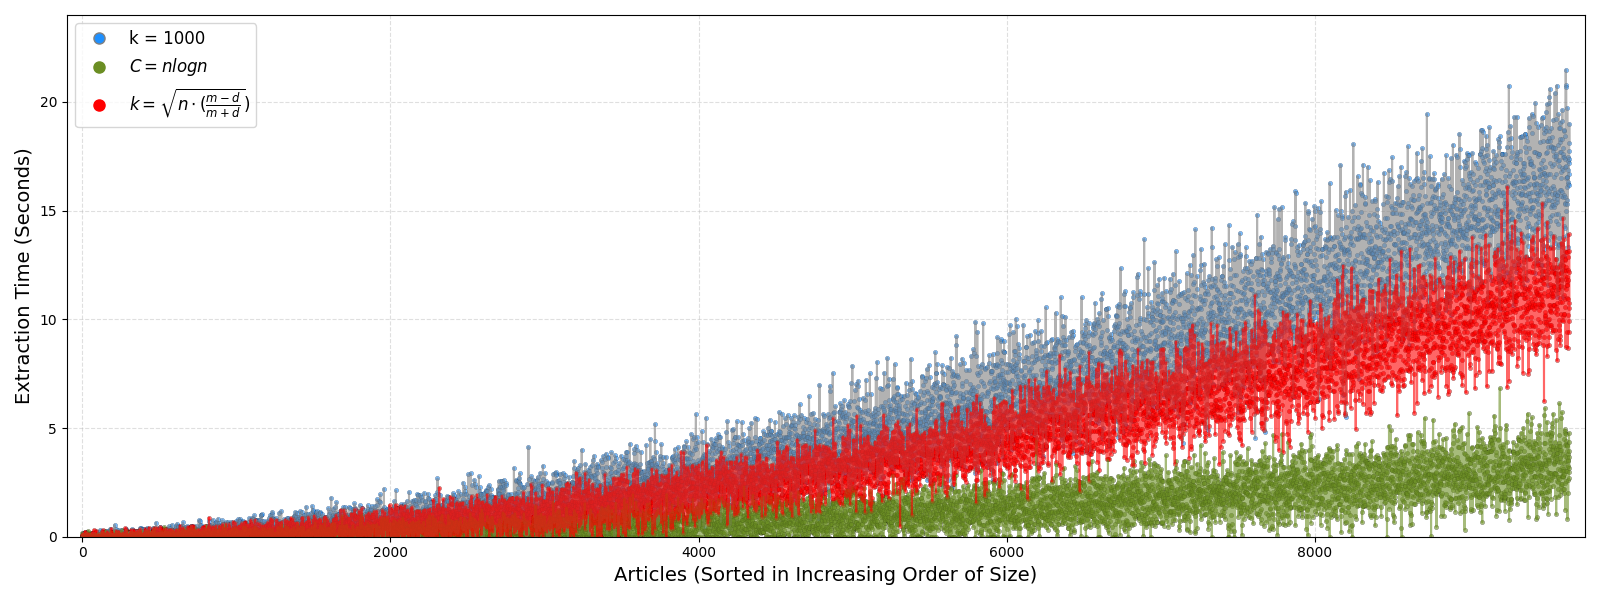
\includegraphics[width=0.9\linewidth]{extraction.png}
        \caption{A plot between articles and aggregate random extraction time}
        \label{fig:top}
    \end{subfigure}

    \vspace{1em}  % spacing between the two subfigures

    \begin{subfigure}{\linewidth}
        \centering
        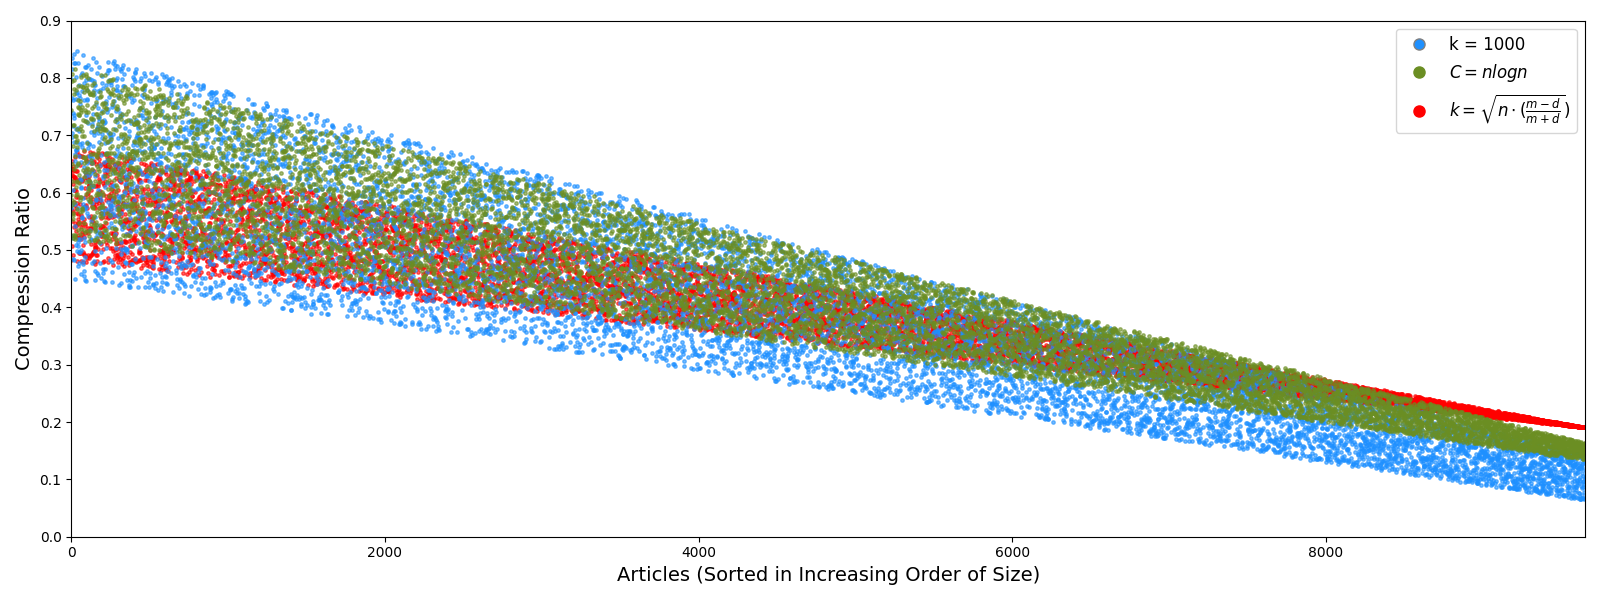
\includegraphics[width=0.9\linewidth]{compression.png}
        \caption{A plot between articles and compressed to original ratio}
        \label{fig:bottom}
    \end{subfigure}

    \caption{Comparison of proposed method with the fixed length method. The X-axis represents the articles sorted based on their sizes. a) Represents the comparison based on the aggregate extraction time of random 100 revisions. b) Represents the comparison based on compressed to original article size ratio.}
    \label{fig:combined}
\end{figure}

\section{Results}
This section begins by presenting high-level descriptive statistics to compare our method across various interval lengths. We treat the case of $k=1000$ as the baseline method and provide a detailed comparison between our approach and the $k=1000$ method proposed by Ferschke et al. Although Verma et al. introduced an online approach to compress the dataset by setting the interval length as $k = \sqrt{n}$, their findings were based on a preliminary analysis and lacked comprehensive evaluation. Therefore, for the purpose of our experiments, we consider $k=1000$ as the baseline state-of-the-art method against which we benchmark our results.


\subsection{Descriptive Results}
Table \ref{tab:compress} presents the aggregate random retrieval time and compression ratio for different values of $k$. Both of our proposed methods significantly outperform the baseline method of $k=1000$ (as introduced by Ferschke et al. \cite{ferschke2011wikipedia}) by a substantial margin. Our approach consistently achieves optimal random revision extraction times without compromising on the compression ratio, across all tested $k$ values. Specifically, using the fixed-length method, we record an average random retrieval time of 0.080 seconds—this is 16 times faster than the baseline $k=1000$, and 1.12 times faster than Verma's method of $k=\sqrt{n}$. In terms of compression, our method maintains a competitive average compression ratio of 0.124, which is only 1.64 times and 1.04 times higher than that achieved by the baseline $k=1000$ and Verma's $k=\sqrt{n}$ methods, respectively. Moreover, our method exhibits a comparatively low standard deviation in random revision extraction time, highlighting its stable and consistent performance across the dataset. On the other hand, we observe a relatively higher standard deviation in the compression ratio. This variation arises primarily because our method tends to estimate a smaller interval length for shorter articles—those with fewer than 500 revisions—thereby increasing the overall compression ratio in such cases. 

However, the results show that optimal compression is performed using the variable-interval length method. Moreover, we observe the optimal compression ratio and revision retrieval time when we fix the \emph{maximum time cost} ($C$) to $nlogn$. The variable-interval length method ( $C = nlogn$) even outperforms the fixed-interval length method in terms of both time (0.07 seconds on average) and space (ratio of 0.128 on average). The reason behind this optimality is the idea of collating all the consecutive minor edits into a single block. Furthermore, given a \emph{maximum time cost}, the method guarantees the optimal compression.

The table also includes the upper and lower bounds for both random revision retrieval time and compression ratio, offering a comprehensive view of performance extremes. Specifically, the values of $k = 2$ and $k = n-1$ serve as the lower and upper bounds for random revision retrieval time, respectively. In contrast, when evaluating compression ratio, the roles of these bounds are reversed: $k = 2$ yields the highest (worst) compression ratio, while $k = n-1$ results in the lowest (best) compression ratio. Although the use of a fixed interval length of $k = 1000$ yields a compression ratio that is close to the theoretical lower bound, it does so at the cost of a higher average random revision retrieval time. This trade-off highlights a limitation of the baseline method. In comparison, our proposed method strikes a more effective balance between time and space efficiency. By dynamically adjusting the interval length, it achieves near-optimal compression while also significantly reducing retrieval time—thus providing a practical and scalable solution for large-scale revision history access.


\subsection{Comparision with the Baseline Method}
Table \ref{tab:compress} presents a comprehensive evaluation of the performance of our proposed model. In this section, we delve into the primary findings reported in Table \ref{tab:compress} and discuss their significance in the context of large-scale Wikipedia revision history analysis. Given that our variable-interval length method consistently outperforms the alternatives, we provide an in-depth comparison between this proposed approach and the widely adopted baseline method, which uses a fixed interval length of $k=1000$. We plot the aggregate random revisions retrieval time and compression ratio for each article in our dataset using both methods. To establish the comparison, we first sorted all the articles in our dataset based on their original sizes (x-axis). This sorting enables us to observe trends and performance patterns across a range of article lengths, making the comparison more insightful.
 
Figure \ref{fig:top} provides a visual comparison between our proposed method and the baseline fixed-interval method ($k=1000$), focusing on two key performance metrics: \emph{random revision retrieval time} and \emph{compression ratio}. As shown in the figure, our method significantly outperforms the $k=1000$ baseline in terms of random revision retrieval time, with a noticeable performance gap across most articles (Fig. \ref{fig:top}). This substantial improvement highlights the efficiency of our approach, especially for larger datasets where retrieval speed becomes increasingly critical.
Additionally, when evaluating the compression ratio on a per-article basis, our method closely mirrors the results achieved by the $k=1000$ method (Fig. \ref{fig:bottom}). This demonstrates that while we gain considerable speed in retrieval, we do not compromise on storage efficiency. A noteworthy observation during our analysis is that out of the total 9652 articles, only 1723 articles contained more than 1000 revisions. This implies that for the majority of articles, where the number of revisions is fewer than 1000, the interval lengths $k=1000$ and $k=n-1$ effectively behave similarly in terms of both revision extraction time and compression ratio. This insight reinforces the motivation behind our work — that is, to develop a more adaptive and scalable approach. It further supports the practicality and relevance of offering an online algorithm that can intelligently adjust to the varying revision history lengths across Wikipedia articles, optimizing both space and time efficiency in the process. 


\begin{figure}
  \centering
  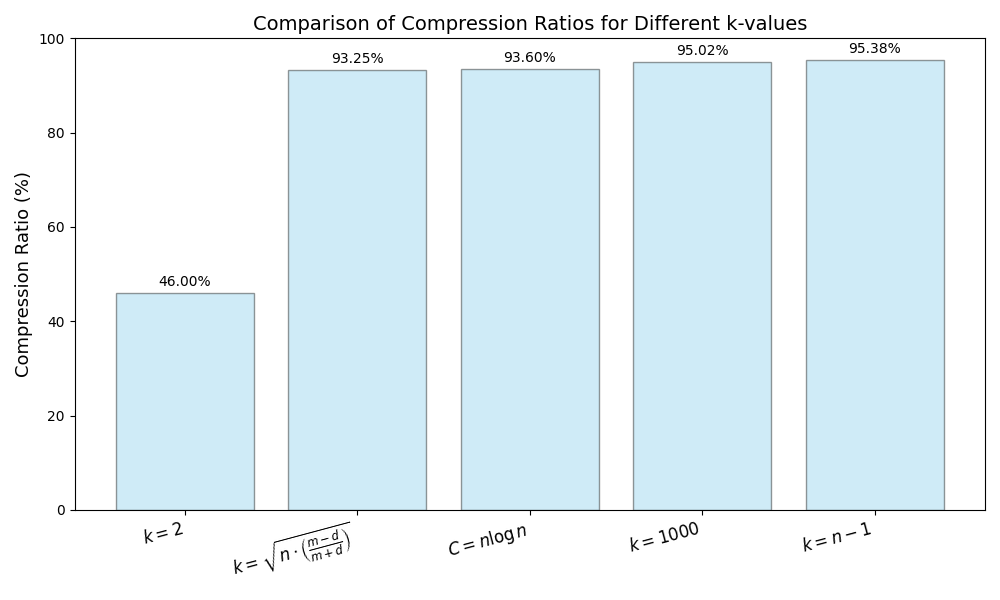
\includegraphics[width=1\linewidth]{overall_compression.png}
  \caption{Overall compression percentage using various interval lengths. $C$ represents the \emph{Maximum Time Cost} for variable-interval length method.}
  \label{fig:over_compre}
\end{figure}

\subsection{Overall Compression}
We also compute the overall compression percentage achieved using our method. We compare our results with the compression achieved using various interval lengths. Fig. \ref{fig:over_compre} shows the compression achieved using different interval lengths. Using the proposed method of interval length estimation, we can reduce the sampled dataset's size to 93.60\% using the variable-interval method and 93.25\% using the fixed-interval method of its original size. Interestingly, the compression achieved using the proposed method is closer to the compression achieved using the baseline method ($k = 1000$). Moreover, the upper bound for compression percentage, i.e., the maximum compression that can be achieved, is 95.38\% (using $k = n-1$), a mare 1.8\% extra reduction from the compression achieved using our method.

Overall, we achieve a comparable compression percentage without compromising on the revision retrieval time. Moreover, the proposed algorithm is scalable, which is an important factor given that the size of the Wikipedia data will increase with time.



\section{Discussion}
Wikipedia is one of the largest online knowledge repositories, and it continues to grow. The number of articles in Wikipedia is increasing by over 17000 a month, with each article having an average of 18.93 revisions~\cite{wiki_stats}. The enormous contribution from millions of editors and the publicly available editing history dataset has made Wikipedia a center of interest for researchers from various domains. However, the extraction of previous edits of Wikipedia articles is a prerequisite for performing various time series analysis. Given the massive size of the Wikipedia edit history dataset, the full edit history analysis of Wikipedia articles is challenging. Moreover, the steady increase in Wikipedia's size will act as a bottleneck in sampling the edits from the full edit history dataset in future analysis.

As discussed before, the compression method proposed by Ferschke et al. provides an elegant way of efficiently representing Wikipedia's full edit history dataset. However, the method relies on a fixed interval length of $k = 1000$, which is not scalable given that Wikipedia's size is continuously increasing. Generally speaking, our results show that fixing the interval length may have an unpredictable effect on per article revision extraction time. Moreover, the sampled dataset reveals that very few articles have more than 1000 revisions (only 1723). This statistic holds for the whole of Wikipedia as the average revisions per article is only 18.93. The small average shows that majority of the Wikipedia articles have comparatively fewer revisions. For instance, out of 6 million English Wikipedia articles, only 5000 have more than 5300 revisions~\cite{wiki_most}. A fixed-length value method for all the articles will inefficiently compress the articles having fewer revisions.  Moreover, we also show that our methods outperform Verma's $k = \sqrt{n}$ method.
 
This paper's proposed methods estimate the interval length based on various parameters such as the number of revisions, the size of each revision, and the difference between two consecutive revisions. The experiment results show that our method efficiently compresses the articles, optimizing both revision retrieval time and space. While designing the compression algorithm, we focused our attention on minimizing the random revision retrieval time as it is a crucial parameter for sampling the set of edits from the full edit history dataset. For example, sampling all the edits of the year 2015 from 1 million compressed articles may require a considerable amount of time if efficient compression is not performed. Moreover, our method is language independent and can be applied to all the language editions of Wikipedia. Overall, we believe that the proposed method will help the researchers perform large-scale Wikipedia analysis without depending on computation power and storage.


\section{Limitations and Future Work}
The results discussed here pertain to the English Wikipedia articles. Moreover, instead of compressing the whole English Wikipedia dataset or the set of most edited articles, we performed experiments on a sample of articles taken from various classes. However, we covered the majority of the classes while performing the stratified sampling. Moreover, the sampled articles provide a brief overview of the English Wikipedia, which could not be possible if a specific set of articles were taken (e.g., most edited articles). Due to stratified sampling, the inference of the results can be generalized on the whole of Wikipedia. 

Secondly, the variable-interval length method relies on finding the optimal partitioning using the dynamic programming paradigm. Given the exponential number of solutions, the time complexity of finding the optimal partitioning is pseudo-polynomial in time~\cite{enwiki:1014657879}. However, the compression task is a one-time process and is easily scalable over the new future revisions. Moreover, there exist polynomial-time approximation algorithms to find the optimal partitioning.
   
Finally, based on our proposed method, we would like to a) develop a python-based toolkit to access the revision edits of Wikipedia articles efficiently and b) provide an open dataset of compressed Wikipedia articles employing the state-of-the-art findings.

\section{Public Release of Dataset And Code}
To encourage further research in this direction, we release the sampled compressed dataset and codes used in the experiments\footnote{https://github.com/descentis/WikECD}. As a part of future work, we also aim to provide all the Wikipedia articles' full revision history in compressed form. Moreover, we plan to create an opensource library to retrieve the edit history from compressed Wikipedia articles efficiently.   


%%
%% The acknowledgments section is defined using the "acks" environment
%% (and NOT an unnumbered section). This ensures the proper
%% identification of the section in the article metadata, and the
%% consistent spelling of the heading.
\begin{acks}
To Robert, for the bagels and explaining CMYK and color spaces.
\end{acks}

%%
%% The next two lines define the bibliography style to be used, and
%% the bibliography file.
\bibliographystyle{ACM-Reference-Format}
\bibliography{sample-base}


%%
%% If your work has an appendix, this is the place to put it.


\end{document}
%%
%% End of file `sample-acmsmall.tex'.
